\documentclass{article}

\usepackage{graphicx}
\usepackage{tikz}
\usepackage{tikzsymbols}
\usetikzlibrary{calc,patterns,shapes.geometric}
\pagestyle{empty}
\usepackage[margin=0pt]{geometry}
\geometry{papersize={14in,12in}}

\def\centerarc[#1](#2)(#3:#4:#5){\draw[#1] ($(#2)+({#5*cos(#3)},{#5*sin(#3)})$) arc (#3:#4:#5);}

\begin{document}
	\begin{figure}
		\centering
		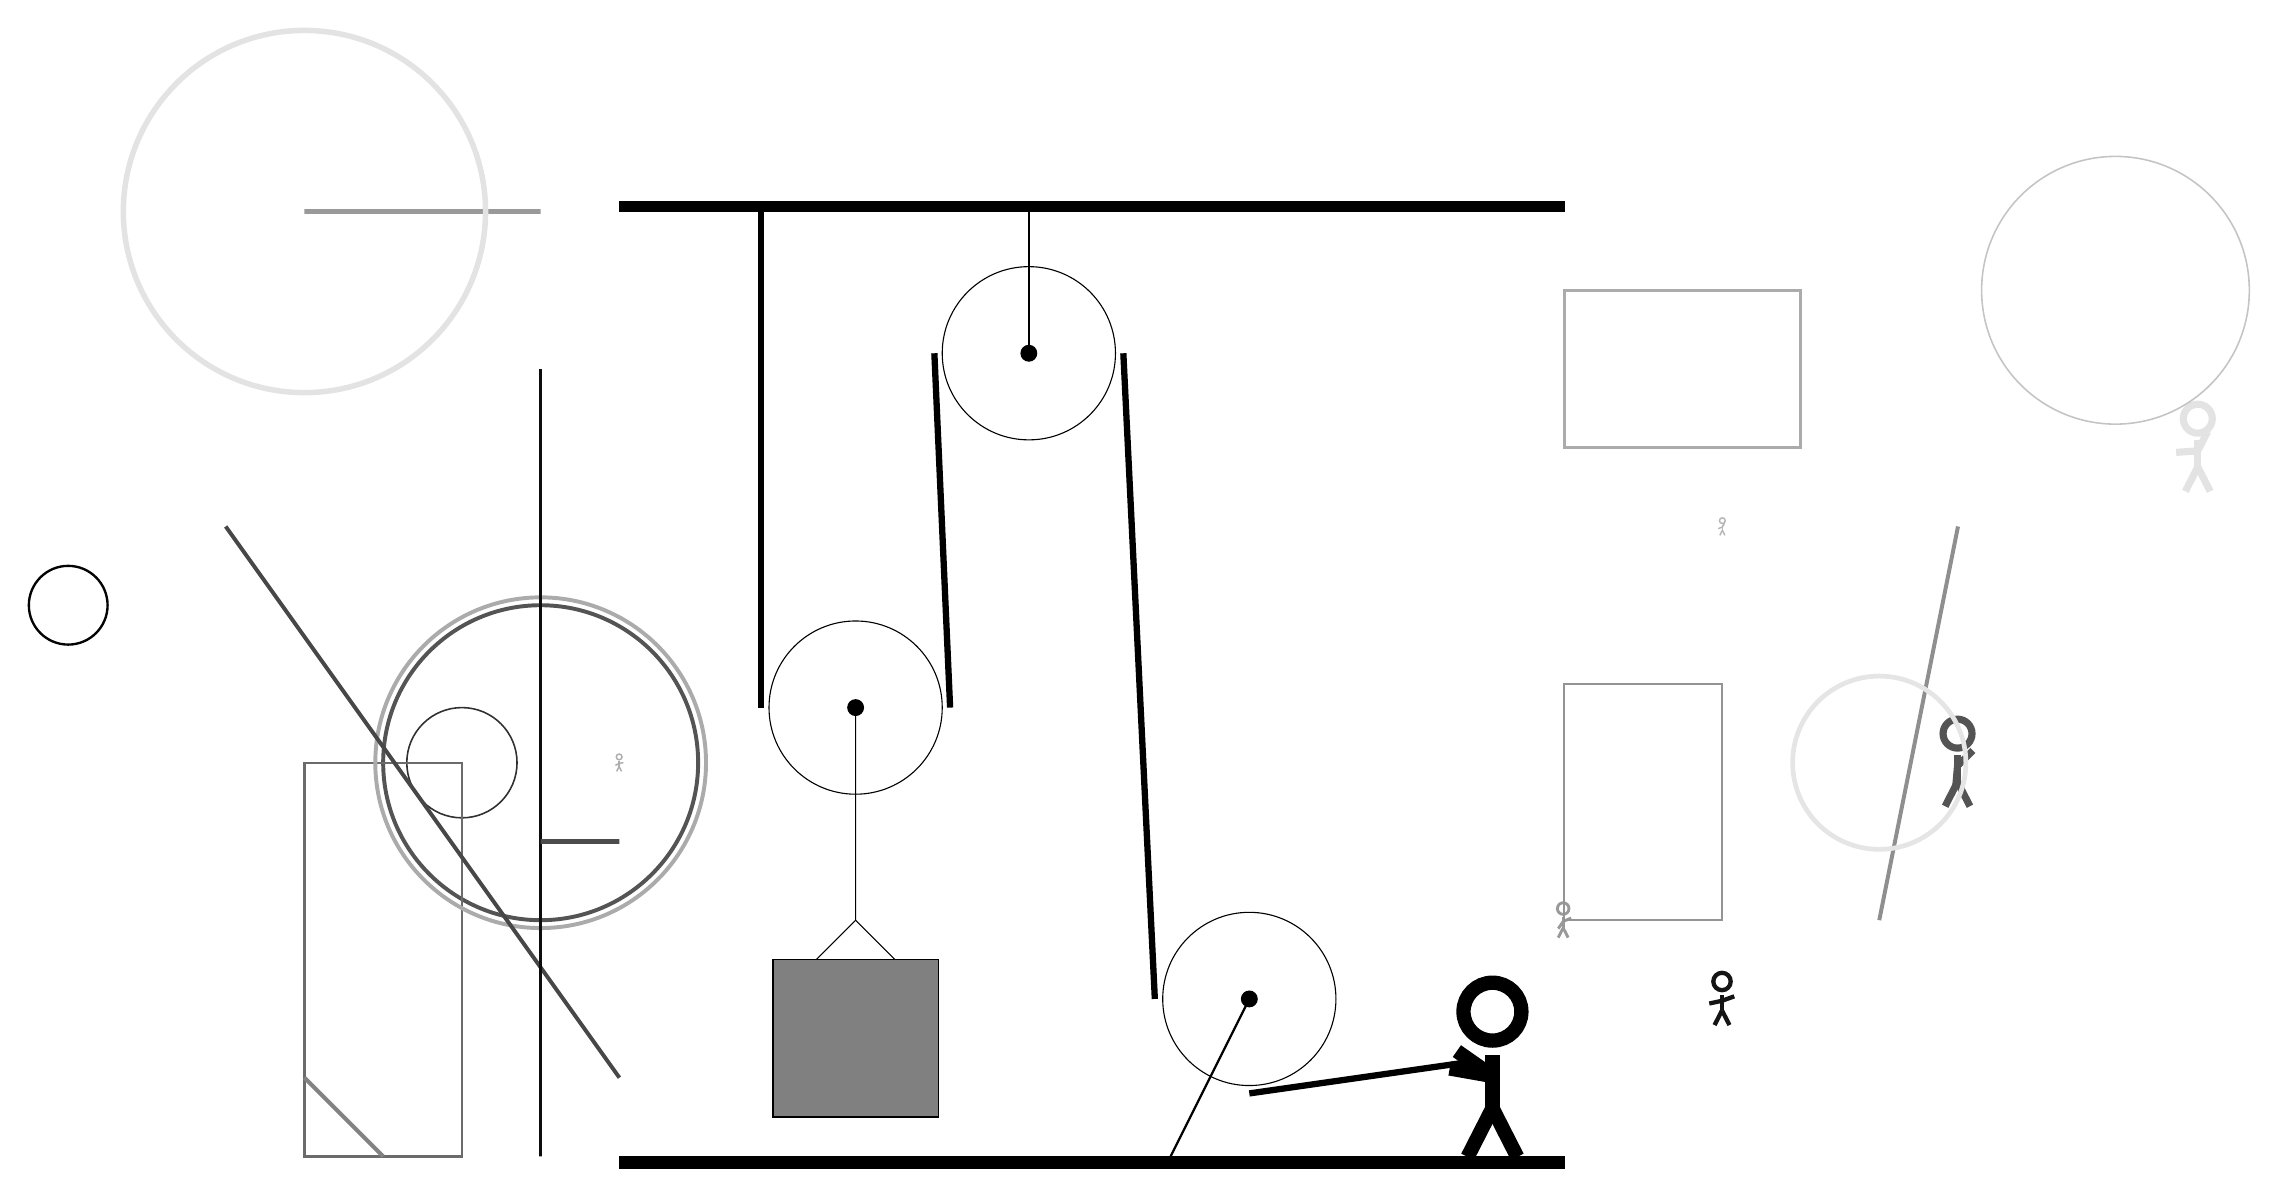
\begin{tikzpicture}
			%%%%% START %%%%%
			
			\draw[fill=black] (-2, 9) rectangle (10, 9.125);
			
			\draw (3.2, 7.2) circle (1.1);
			\draw[fill=black] (3.2, 7.2) circle (0.1);
			\draw[thick] (3.2, 7.2) -- (3.2, 9);
			
			\draw (6, -1) circle (1.1);
			\draw[fill=black] (6, -1) circle (0.1);
			\draw[thick] (6, -1) -- (5, -3);
			
			\draw (1, 2.7) circle (1.1);
			\draw[fill=black] (1, 2.7) circle (0.1);
			
			\draw (1, 2.7) -- (1, 0) -- (0.5, -0.5);
			\draw (1, 0) -- (1.5, -0.5);
			\draw[fill=black!50] (-0.05, -0.5) rectangle (2.05, -2.5);
			
			\draw [line width=0.2mm, color=black!81](-4, 2) circle (0.7);
			
			\node[line width=0.2mm, color=black!32] at (-2, 2) {\Strichmaxerl[1][29][9]};
			\draw[line width=0.5mm, color=black!44](15, 5) -- (14, 0);
			\draw [line width=0.3mm, color=black!99](-9, 4) circle (0.5);
			\node[line width=0.6mm, color=black!40] at (10, 0) {\Strichmaxerl[2][56][23]};
			\draw [line width=0.5mm, color=black!67](-3, 2) circle (2.0);
			\draw[line width=0.3mm, color=black!42] (12, 3) rectangle (10, 0);
			\draw[line width=0.3mm, color=black!58] (-4, -3) rectangle (-6, 2);
			\node[line width=0.6mm, color=black!11] at (18, 6) {\Strichmaxerl[5][4][63]};
			
			\draw[line width=0.7mm, color=black!40] (-3, 9) rectangle (-6, 9);
			
			\draw [line width=0.5mm, color=black!33](-3, 2) circle (2.1);
			\draw[line width=0.4mm, color=black!33] (10, 6) rectangle (13, 8);
			\node[line width=0.6mm, color=black!92] at (12, -1) {\Strichmaxerl[3][12][20]};
			
			\draw[line width=0.3mm, color=black!40] (-3, 1) rectangle (-3, 7);
			\node[line width=0.2mm, color=black!29] at (12, 5) {\Strichmaxerl[1][20][62]};
			\draw[line width=0.5mm, color=black!72](-7, 5) -- (-2, -2);
			
			\node[line width=0.6mm, color=black!67] at (15, 2) {\Strichmaxerl[5][85][45]};
			
			\draw [line width=0.6mm, color=black!10](14, 2) circle (1.1);
			\draw[line width=0.5mm, color=black!49](-5, -3) -- (-6, -2);
			
			\draw[line width=0.4mm, color=black!95] (-3, 7) rectangle (-3, -3);
			\draw [line width=0.7mm, color=black!11](-6, 9) circle (2.3);
			
			\draw [line width=0.2mm, color=black!23](17, 8) circle (1.7);
			
			\draw[line width=0.7mm, color=black!70] (-2, 1) rectangle (-3, 1);
			
			\draw[line width=0.8mm] (-0.2, 9) -- (-0.2, 2.7);
			\centerarc[line width=0.8mm](1, 2.7)(180:360:1.2000000000000002);
			\draw[line width=0.8mm](2.2, 2.7) -- (2.0, 7.2);
			\centerarc[line width=0.8mm](3.2, 7.2)(0:180:1.2000000000000002);
			\draw[line width=0.8mm](4.4, 7.2) -- (4.8, -1);
			\centerarc[line width=0.8mm](6, -1)(180:270:1.2000000000000002);
			\draw[line width=0.8mm](6, -2.2) -- (8.8, -1.8);
			
			\node at (9, -1.9) {\Strichmaxerl[10][-35][170]};
			
			\draw[fill=black] (-2, -3) rectangle (10, -3.15);
			
			%%%%% END %%%%%
		\end{tikzpicture}
	\end{figure}	
\end{document}